\documentclass{article}\usepackage[]{graphicx}\usepackage[]{xcolor}
% maxwidth is the original width if it is less than linewidth
% otherwise use linewidth (to make sure the graphics do not exceed the margin)
\makeatletter
\def\maxwidth{ %
  \ifdim\Gin@nat@width>\linewidth
    \linewidth
  \else
    \Gin@nat@width
  \fi
}
\makeatother

\definecolor{fgcolor}{rgb}{0.345, 0.345, 0.345}
\newcommand{\hlnum}[1]{\textcolor[rgb]{0.686,0.059,0.569}{#1}}%
\newcommand{\hlsng}[1]{\textcolor[rgb]{0.192,0.494,0.8}{#1}}%
\newcommand{\hlcom}[1]{\textcolor[rgb]{0.678,0.584,0.686}{\textit{#1}}}%
\newcommand{\hlopt}[1]{\textcolor[rgb]{0,0,0}{#1}}%
\newcommand{\hldef}[1]{\textcolor[rgb]{0.345,0.345,0.345}{#1}}%
\newcommand{\hlkwa}[1]{\textcolor[rgb]{0.161,0.373,0.58}{\textbf{#1}}}%
\newcommand{\hlkwb}[1]{\textcolor[rgb]{0.69,0.353,0.396}{#1}}%
\newcommand{\hlkwc}[1]{\textcolor[rgb]{0.333,0.667,0.333}{#1}}%
\newcommand{\hlkwd}[1]{\textcolor[rgb]{0.737,0.353,0.396}{\textbf{#1}}}%
\let\hlipl\hlkwb

\usepackage{framed}
\makeatletter
\newenvironment{kframe}{%
 \def\at@end@of@kframe{}%
 \ifinner\ifhmode%
  \def\at@end@of@kframe{\end{minipage}}%
  \begin{minipage}{\columnwidth}%
 \fi\fi%
 \def\FrameCommand##1{\hskip\@totalleftmargin \hskip-\fboxsep
 \colorbox{shadecolor}{##1}\hskip-\fboxsep
     % There is no \\@totalrightmargin, so:
     \hskip-\linewidth \hskip-\@totalleftmargin \hskip\columnwidth}%
 \MakeFramed {\advance\hsize-\width
   \@totalleftmargin\z@ \linewidth\hsize
   \@setminipage}}%
 {\par\unskip\endMakeFramed%
 \at@end@of@kframe}
\makeatother

\definecolor{shadecolor}{rgb}{.97, .97, .97}
\definecolor{messagecolor}{rgb}{0, 0, 0}
\definecolor{warningcolor}{rgb}{1, 0, 1}
\definecolor{errorcolor}{rgb}{1, 0, 0}
\newenvironment{knitrout}{}{} % an empty environment to be redefined in TeX

\usepackage{alltt}
\usepackage[margin=1.0in]{geometry} % To set margins
\usepackage{amsmath}  % This allows me to use the align functionality.
                      % If you find yourself trying to replicate
                      % something you found online, ensure you're
                      % loading the necessary packages!
\usepackage{amsfonts} % Math font
\usepackage{fancyvrb}
\usepackage{hyperref} % For including hyperlinks
\usepackage[shortlabels]{enumitem}% For enumerated lists with labels specified
                                  % We had to run tlmgr_install("enumitem") in R
\usepackage{float}    % For telling R where to put a table/figure
\usepackage{natbib}        %For the bibliography
\bibliographystyle{apalike}%For the bibliography
\IfFileExists{upquote.sty}{\usepackage{upquote}}{}
\begin{document}


\cite{Kasdin25} show that dopamine in the brains of young zebra finches acts as 
a learning signal, increasing when they sing closer to their adult song and 
decreasing when they sing further away, effectively guiding their vocal 
development through trial-and-error. This suggests that complex natural 
behaviors, like learning to sing, are shaped by dopamine-driven reinforcement 
learning, similar to how artificial intelligence learns. You can find the 
paper at this link:
\href{https://www.nature.com/articles/s41586-025-08729-1}{{https://www.nature.com/articles/s41586-025-08729-1}.}.

Note they measure dopamine using fibre photometry, changes in the fluorescence
indicate dopamine changes in realtime. Their specific measurement considers 
changes in flourescence in 100-ms windows between 200 and 300 ms from the start 
of singing, averaged across development.

\begin{enumerate}
%%%%%%%%%%%%%%%%%%%%%%%%%%%%%%%%%%%%%%%%%%%%%%%%%%%%%%%%%%%%%%%%%
% CONDUCT A POWER ANALYSIS
%%%%%%%%%%%%%%%%%%%%%%%%%%%%%%%%%%%%%%%%%%%%%%%%%%%%%%%%%%%%%%%%%
\item Using the \texttt{pwr} package for \texttt{R} \citep{pwr},
conduct a power analysis. How many observations would the researchers 
need to detect a moderate-to-large effect ($d=0.65$) when using 
$\alpha=0.05$ and default power (0.80) for a two-sided one sample 
$t$ test. \\
\begin{knitrout}
\definecolor{shadecolor}{rgb}{0.969, 0.969, 0.969}\color{fgcolor}\begin{kframe}
\begin{alltt}
\hldef{alpha} \hlkwb{<-} \hlnum{0.05}
\hldef{(pwr.analysis} \hlkwb{<-} \hlkwd{pwr.t.test}\hldef{(}\hlkwc{d}\hldef{=}\hlnum{0.65}\hldef{,} \hlkwc{sig.level} \hldef{= alpha,} \hlkwc{power} \hldef{=} \hlnum{0.80}\hldef{,}
                            \hlkwc{type} \hldef{=} \hlsng{"one.sample"}\hldef{,} \hlkwc{alternative} \hldef{=} \hlsng{"two.sided"}\hldef{))}
\end{alltt}
\begin{verbatim}
## 
##      One-sample t test power calculation 
## 
##               n = 20.58039
##               d = 0.65
##       sig.level = 0.05
##           power = 0.8
##     alternative = two.sided
\end{verbatim}
\end{kframe}
\end{knitrout}
\textbf{Solution:} Using the \verb|pwr.t.test()| function from the \texttt{pwr} package, the number of observations the researchers would need is $n = 20.58$. In this study, the researchers used $n=25$ observation, well over the number of observations necessary.
%%%%%%%%%%%%%%%%%%%%%%%%%%%%%%%%%%%%%%%%%%%%%%%%%%%%%%%%%%%%%%%%%
% COLLECT DATA
%%%%%%%%%%%%%%%%%%%%%%%%%%%%%%%%%%%%%%%%%%%%%%%%%%%%%%%%%%%%%%%%%
\item Click the link to go to the paper. Find the source data for 
Figure 2. Download the Excel file. Describe what you needed to
do to collect the data for Figure 2(g). Note that you only need the 
\texttt{closer\_vals} and \texttt{further\_vals}. Ensure to 
\texttt{mutate()} the data to get a difference 
(e.g., \texttt{closer\_vals - further\_vals}).
\begin{knitrout}
\definecolor{shadecolor}{rgb}{0.969, 0.969, 0.969}\color{fgcolor}\begin{kframe}
\begin{alltt}
\hlcom{# closer vals}
\hldef{closer.data} \hlkwb{<-} \hlkwd{read_csv}\hldef{(}\hlsng{"closer_vals.csv"}\hldef{)}
\hlcom{# further vals}
\hldef{further.data} \hlkwb{<-} \hlkwd{read_csv}\hldef{(}\hlsng{"further_vals.csv"}\hldef{)}

\hlcom{# consolidate all data}
\hldef{figG.data} \hlkwb{<-} \hlkwd{tibble}\hldef{(}\hlkwc{closer_vals} \hldef{= closer.data}\hlopt{$}\hldef{closer_vals,}
                    \hlkwc{further_vals} \hldef{= further.data}\hlopt{$}\hldef{further_vals) |>}
  \hlkwd{mutate}\hldef{(}\hlkwc{val_diffs} \hldef{= closer_vals} \hlopt{-} \hldef{further_vals)}
\hlcom{# create table for sweave}
\hlkwd{xtable}\hldef{(figG.data)}
\end{alltt}
\end{kframe}
\end{knitrout}
\textbf{Solution:} The code snippet above shows the code used for creating the table and generating the table (Table \ref{table1}) shown on the next page, using \texttt{xtable} \citep{xtable}.
\begin{table}[ht]
\centering
\begin{tabular}{rrrr}
  \hline
 observation & closer\_vals & further\_vals & val\_diffs \\ 
  \hline
  1 & 0.28 & -0.19 & 0.47 \\ 
  2 & 0.08 & -0.03 & 0.11 \\ 
  3 & 0.13 & -0.19 & 0.32 \\ 
  4 & 0.04 & -0.07 & 0.11 \\ 
  5 & 0.15 & -0.09 & 0.23 \\ 
  6 & 0.20 & -0.16 & 0.36 \\ 
  7 & 0.16 & -0.31 & 0.47 \\ 
  8 & 0.18 & -0.16 & 0.34 \\ 
  9 & 0.13 & -0.13 & 0.26 \\ 
  10 & 0.10 & -0.05 & 0.15 \\ 
  11 & 0.33 & -0.60 & 0.93 \\ 
  12 & 0.17 & -0.24 & 0.41 \\ 
  13 & 0.07 & -0.12 & 0.20 \\ 
  14 & 0.00 & -0.13 & 0.13 \\ 
  15 & 0.00 & -0.04 & 0.04 \\ 
  16 & 0.09 & -0.24 & 0.33 \\ 
  17 & 0.26 & -0.34 & 0.61 \\ 
  18 & 0.28 & -0.31 & 0.59 \\ 
  19 & 0.07 & -0.18 & 0.25 \\ 
  20 & 0.15 & -0.07 & 0.23 \\ 
  21 & 0.27 & -0.34 & 0.61 \\ 
  22 & 0.15 & -0.19 & 0.34 \\ 
  23 & 0.10 & -0.20 & 0.30 \\ 
  24 & 0.19 & -0.31 & 0.50 \\ 
  25 & 0.34 & -0.35 & 0.69 \\ 
   \hline
\end{tabular}
\caption{Table showing values for \texttt{closer\_vals}, \texttt{further\_vals}, and their corresponding differences (\texttt{val\_diffs}).}
\label{table1}
\end{table}
\newpage
%%%%%%%%%%%%%%%%%%%%%%%%%%%%%%%%%%%%%%%%%%%%%%%%%%%%%%%%%%%%%%%%%
% SUMMARIZE DATA
%%%%%%%%%%%%%%%%%%%%%%%%%%%%%%%%%%%%%%%%%%%%%%%%%%%%%%%%%%%%%%%%%
\item Summarize the data.
\begin{enumerate}
  \item Summarize the further data. Do the data suggest that
   dopamine in the brains of young zebra finches decreases when
   they sing further away?
\begin{knitrout}
\definecolor{shadecolor}{rgb}{0.969, 0.969, 0.969}\color{fgcolor}\begin{kframe}
\begin{alltt}
\hlcom{# part A}
\hldef{further.summary} \hlkwb{<-} \hlkwd{summarize}\hldef{(figG.data,}
                         \hlkwc{mean} \hldef{=} \hlkwd{mean}\hldef{(further_vals),}
                         \hlkwc{variance} \hldef{=} \hlkwd{var}\hldef{(further_vals),}
                         \hlkwc{median} \hldef{=} \hlkwd{median}\hldef{(further_vals),}
                         \hlkwc{IQR} \hldef{=} \hlkwd{IQR}\hldef{(further_vals),}
                         \hlkwc{skewness} \hldef{=} \hlkwd{skewness}\hldef{(further_vals),}
                         \hlkwc{e.kurtosis} \hldef{=} \hlkwd{kurtosis}\hldef{(further_vals))}
\hlkwd{xtable}\hldef{(further.summary)}
\end{alltt}
\end{kframe}
\end{knitrout}
\textbf{Solution:} Above is a code snippet used to generate a table of summary statistics (Table \ref{table2}) for the further data. Since the mean and median are both negative, this suggests that dopamine is decreasing for further values. Some functions used to calculate summary statistics came from the \texttt{e1071} \citep{e1071} package.
\begin{table}[ht]
\centering
\begin{tabular}{rrrrrrr}
  \hline
 mean & variance & median & IQR & skewness & e.kurtosis \\ 
  \hline
-0.20 & 0.02 & -0.19 & 0.19 & -1.04 & 1.19 \\ 
   \hline
\end{tabular}
\caption{Summary Statistics for further data.}
\label{table2}
\end{table}
   \item Summarize the closer data. Do the data suggest that
   dopamine in the brains of young zebra finches increases when
   they sing closer to their adult song?
\begin{knitrout}
\definecolor{shadecolor}{rgb}{0.969, 0.969, 0.969}\color{fgcolor}\begin{kframe}
\begin{alltt}
 \hlcom{# part B}
 \hldef{closer.summary} \hlkwb{<-} \hlkwd{summarize}\hldef{(figG.data,}
                          \hlkwc{mean} \hldef{=} \hlkwd{mean}\hldef{(closer_vals),}
                          \hlkwc{variance} \hldef{=} \hlkwd{var}\hldef{(closer_vals),}
                          \hlkwc{median} \hldef{=} \hlkwd{median}\hldef{(closer_vals),}
                          \hlkwc{IQR} \hldef{=} \hlkwd{IQR}\hldef{(closer_vals),}
                          \hlkwc{skewness} \hldef{=} \hlkwd{skewness}\hldef{(closer_vals),}
                          \hlkwc{e.kurtosis} \hldef{=} \hlkwd{kurtosis}\hldef{(closer_vals))}
 \hlkwd{xtable}\hldef{(closer.summary)}
\end{alltt}
\end{kframe}
\end{knitrout}
  \textbf{Solution:} Above is a code snippet used to generate a table of summary statistics (Table \ref{table3}) for the closer data. Since the mean and median are both positive, this suggests that dopamine is increasing for closer values. 
\begin{table}[ht]
\centering
\begin{tabular}{rrrrrrr}
  \hline
 mean & variance & median & IQR & skewness & e.kurtosis \\ 
  \hline
 0.16 & 0.01 & 0.15 & 0.11 & 0.30 & -0.86 \\ 
   \hline
\end{tabular}
\caption{Summary Statistics for closer data.}
\label{table3}
\end{table}
  \item Summarize the paired differences. Do the data suggest
  that there is a difference between dopamine in the brains of
  young zebra finches when they sing further away compared to 
  closer to their adult song?

\textbf{Solution:} Above is a code snippet used to generate a table of summary statistics (Table \ref{table4}) for the paired differences. Since the mean and median are both positive, this suggests that dopamine is changing in paired differences.
\begin{table}[ht]
\centering
\begin{tabular}{rrrrrrr}
  \hline
  mean & variance & median & IQR & skewness & e.kurtosis \\ 
  \hline
  0.36 & -0.01 & 0.33 & -0.08 & 1.33 & -2.05 \\ 
   \hline
\end{tabular}
\caption{Summary Statistics for paired differences.}
\label{table4}
\end{table}
  \item \textbf{Optional Challenge:} Can you reproduce Figure 2(g)?
  Note that the you can use \texttt{geom\_errorbar()} to plot
  the range created by adding the mean $\pm$ one standard deviation.
\end{enumerate}
%%%%%%%%%%%%%%%%%%%%%%%%%%%%%%%%%%%%%%%%%%%%%%%%%%%%%%%%%%%%%%%%%
% CONDUCT THE TESTS
%%%%%%%%%%%%%%%%%%%%%%%%%%%%%%%%%%%%%%%%%%%%%%%%%%%%%%%%%%%%%%%%%
\item Conduct the inferences they do in the paper. Make sure to report the results
a little more comprehensively -- that is your parenthetical should look something
like: ($t=23.99$, $p<0.0001$; $g=1.34$; 95\% CI: 4.43, 4.60).\\
\textbf{Note:} Your numbers may vary slightly as they performed some unclear
correction of their $p$-values. I'm waiting to hear back from them via email!
\begin{enumerate}
  \item ``The close responses differed significantly from 0 ($p=1.63 \times 10^{-8}$).''
\begin{knitrout}
\definecolor{shadecolor}{rgb}{0.969, 0.969, 0.969}\color{fgcolor}\begin{kframe}
\begin{alltt}
\hlcom{# part A (closer)}
\hldef{mu0} \hlkwb{<-} \hlnum{0}
\hldef{x.closer} \hlkwb{<-} \hldef{figG.data}\hlopt{$}\hldef{closer_vals}

\hlcom{# hedge's g + CI}
\hlkwd{hedges_g}\hldef{(}\hlkwc{x} \hldef{= x.closer,} \hlkwc{mu} \hldef{= mu0,} \hlkwc{alternative} \hldef{=} \hlsng{"greater"}\hldef{)}
\end{alltt}
\begin{verbatim}
## Hedges' g |      95% CI
## -----------------------
## 1.61      | [1.10, Inf]
## 
## - One-sided CIs: upper bound fixed at [Inf].
\end{verbatim}
\begin{alltt}
\hlkwd{interpret_hedges_g}\hldef{(}\hlnum{1.61}\hldef{)}
\end{alltt}
\begin{verbatim}
## [1] "large"
## (Rules: cohen1988)
\end{verbatim}
\begin{alltt}
\hlcom{# t.test}
\hlkwd{t.test}\hldef{(}\hlkwc{x}\hldef{=x.closer,} \hlkwc{mu} \hldef{= mu0,} \hlkwc{alternative} \hldef{=} \hlsng{"greater"}\hldef{)}
\end{alltt}
\begin{verbatim}
## 
## 	One Sample t-test
## 
## data:  x.closer
## t = 8.3024, df = 24, p-value = 8.132e-09
## alternative hypothesis: true mean is greater than 0
## 95 percent confidence interval:
##  0.1240301       Inf
## sample estimates:
## mean of x 
## 0.1562231
\end{verbatim}
\end{kframe}
\end{knitrout}
\textbf{Solution:} Since we expect dopamine levels to increase when the responses are closer, we want to use a right-tailed test. This givens us the results: 
\begin{center}
($t = 8.30$; $p = 8.13 * 10^{-9}$; $g = 1.61$; $95\%$ CI: 0.124, Inf)
\end{center}
The functions used to accomplish these tasks (\verb|hedges_g(), t.test()|), came from the \texttt{effectsize} \citep{effectsize} package. 

  \item ``The far responses differed significantly from 0 ($p=5.17 \times 10^{-8}$).''
\begin{knitrout}
\definecolor{shadecolor}{rgb}{0.969, 0.969, 0.969}\color{fgcolor}\begin{kframe}
\begin{alltt}
\hlcom{# part B (further)}
\hldef{mu0} \hlkwb{<-} \hlnum{0}
\hldef{x.further} \hlkwb{<-} \hldef{figG.data}\hlopt{$}\hldef{further_vals}

\hlcom{# hedge's g + CI}
\hlkwd{hedges_g}\hldef{(}\hlkwc{x} \hldef{= x.further,} \hlkwc{mu} \hldef{= mu0,} \hlkwc{alternative} \hldef{=} \hlsng{"less"}\hldef{)}
\end{alltt}
\begin{verbatim}
## Hedges' g |        95% CI
## -------------------------
## -1.51     | [-Inf, -1.02]
## 
## - One-sided CIs: lower bound fixed at [-Inf].
\end{verbatim}
\begin{alltt}
\hlkwd{interpret_hedges_g}\hldef{(}\hlopt{-}\hlnum{1.51}\hldef{)}
\end{alltt}
\begin{verbatim}
## [1] "large"
## (Rules: cohen1988)
\end{verbatim}
\begin{alltt}
\hlcom{# t.test}
\hlkwd{t.test}\hldef{(}\hlkwc{x}\hldef{=x.further,} \hlkwc{mu} \hldef{= mu0,} \hlkwc{alternative} \hldef{=} \hlsng{"less"}\hldef{)}
\end{alltt}
\begin{verbatim}
## 
## 	One Sample t-test
## 
## data:  x.further
## t = -7.778, df = 24, p-value = 2.587e-08
## alternative hypothesis: true mean is less than 0
## 95 percent confidence interval:
##        -Inf -0.1581322
## sample estimates:
##  mean of x 
## -0.2027244
\end{verbatim}
\end{kframe}
\end{knitrout}
\textbf{Solution:} Since we expect dopamine levels to decrease when the responses are further, we want to use a left-tailed test. This givens us the results: 
\begin{center}
($t = -7.78$; $p = 2.59 * 10^{-8}$; $g = -1.51$; $95\%$ CI: -Inf, -0.158)
\end{center}
  \item ``The difference between populations was significant ($p=1.04 \times10^{-8}$).''
\begin{knitrout}
\definecolor{shadecolor}{rgb}{0.969, 0.969, 0.969}\color{fgcolor}\begin{kframe}
\begin{alltt}
\hlcom{# part C (differences)}
\hldef{mu0} \hlkwb{<-} \hlnum{0}
\hldef{x.diff} \hlkwb{<-} \hldef{figG.data}\hlopt{$}\hldef{val_diffs}

\hlcom{# hedge's g + CI}
\hlkwd{hedges_g}\hldef{(}\hlkwc{x} \hldef{= x.diff,} \hlkwc{mu} \hldef{= mu0,} \hlkwc{alternative} \hldef{=} \hlsng{"two.sided"}\hldef{)}
\end{alltt}
\begin{verbatim}
## Hedges' g |       95% CI
## ------------------------
## 1.65      | [1.04, 2.24]
\end{verbatim}
\begin{alltt}
\hlkwd{interpret_hedges_g}\hldef{(}\hlnum{1.65}\hldef{)}
\end{alltt}
\begin{verbatim}
## [1] "large"
## (Rules: cohen1988)
\end{verbatim}
\begin{alltt}
\hlcom{# t.test}
\hlkwd{t.test}\hldef{(}\hlkwc{x}\hldef{=x.diff,} \hlkwc{mu} \hldef{= mu0,} \hlkwc{alternative} \hldef{=} \hlsng{"two.sided"}\hldef{)}
\end{alltt}
\begin{verbatim}
## 
## 	One Sample t-test
## 
## data:  x.diff
## t = 8.5109, df = 24, p-value = 1.037e-08
## alternative hypothesis: true mean is not equal to 0
## 95 percent confidence interval:
##  0.2719028 0.4459921
## sample estimates:
## mean of x 
## 0.3589475
\end{verbatim}
\end{kframe}
\end{knitrout}
\textbf{Solution:} Since we expect the difference to be significant between populations, we want to use a two-tailed test. This givens us the results: 
\begin{center}
($t = 8.51$; $p = 1.04 * 10^{-8}$; $g = 1.65$; $95\%$ CI: 0.272, 0.446)
\end{center}

\end{enumerate}
\newpage
%%%%%%%%%%%%%%%%%%%%%%%%%%%%%%%%%%%%%%%%%%%%%%%%%%%%%%%%%%%%%%%%%
% CONDUCT THE TESTS
%%%%%%%%%%%%%%%%%%%%%%%%%%%%%%%%%%%%%%%%%%%%%%%%%%%%%%%%%%%%%%%%%
\item Reverse engineer the hypothesis test plot from Lecture 20 to create accurate
hypothesis testing plots for each part of the previous question.
\begin{enumerate}
  \item Question 4, part(a).
\begin{figure}[H]
 \begin{center}
\begin{knitrout}
\definecolor{shadecolor}{rgb}{0.969, 0.969, 0.969}\color{fgcolor}
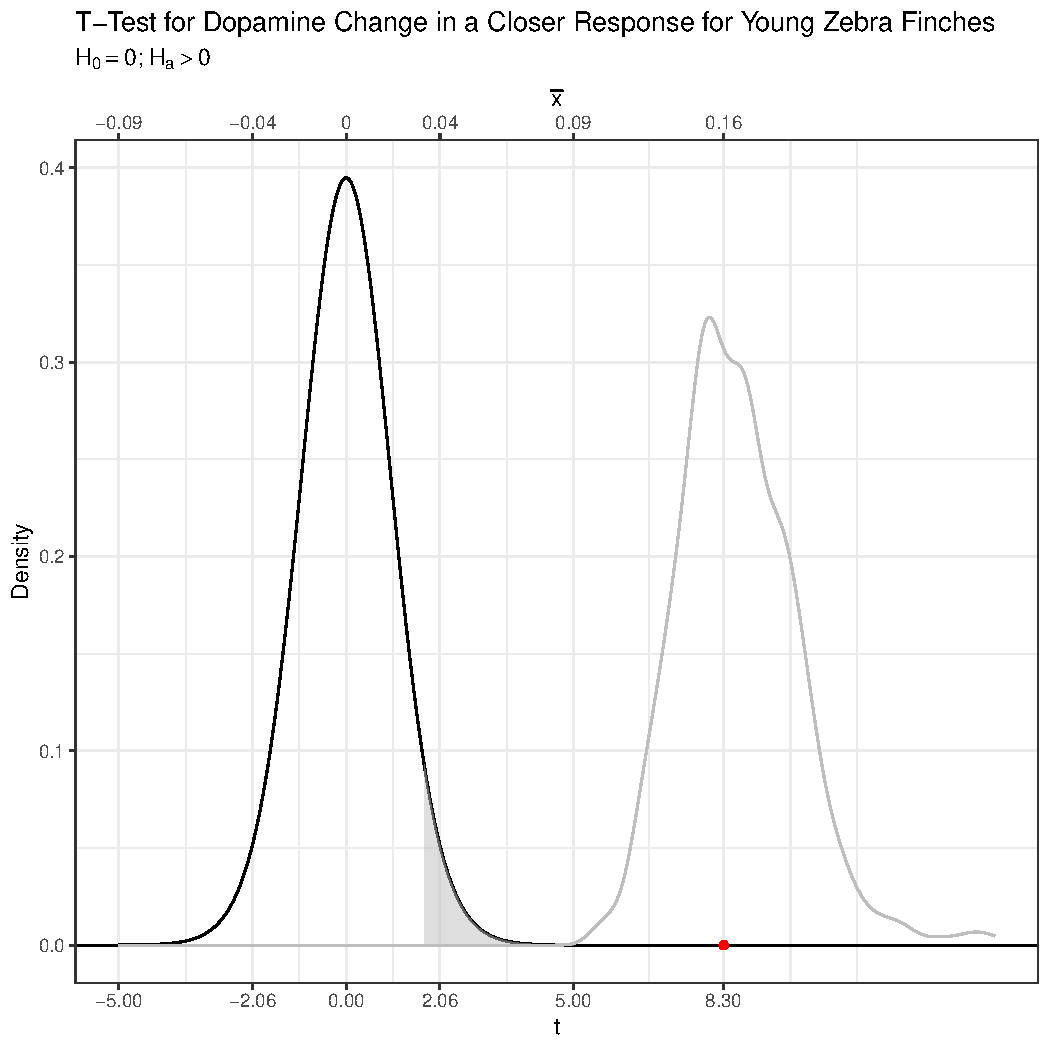
\includegraphics[width=\maxwidth]{figure/unnamed-chunk-10-1} 
\end{knitrout}
\caption{A figure showing the T-Test for Dopamine change in closer responses.}
 \end{center}
 \end{figure}  
 \newpage
  \item Question 4, part(b).
  \begin{figure}[H]
 \begin{center}
\begin{knitrout}
\definecolor{shadecolor}{rgb}{0.969, 0.969, 0.969}\color{fgcolor}\begin{kframe}


{\ttfamily\noindent\bfseries\color{errorcolor}{\#\# Error in `geom\_ribbon()`:\\\#\# ! Problem while converting geom to grob.\\\#\# i Error occurred in the 4th layer.\\\#\# Caused by error:\\\#\# ! Unknown colour name: reg}}\end{kframe}
\end{knitrout}
\caption{A figure showing the T-Test for Dopamine change in further responses.}
 \end{center}
 \end{figure}  
%   \item Question 4, part(c).
%   \begin{figure}[H]
%  \begin{center}
% <<echo = F, message=FALSE, warning=FALSE, fig.dim = c(6,5)>>=
% # diff data
% s.diff <- sd(x.diff)
% xbar.diff <- mean(x.diff)
% t.stat.diff <- (xbar.diff - mu0)/(s.diff/sqrt(n))
% 
% # For plotting the observed point
% ggdat.obs.diff <- tibble(t    = t.stat.diff, 
%                             y    = 0) # to plot on x-axis
% 
% # Resampling to approximate the sampling distribution 
% # on the data
% R <- 1000
% resamples <- tibble(t=numeric(R))
% for(i in 1:R){
%   curr.sample <- sample(x=x.diff,
%                         size=n,
%                         replace=T)
%   resamples$t[i] = (mean(curr.sample)-mu0)/(sd(curr.sample)/sqrt(n))
% }
% 
% t.breaks.diff <- c(-5, qt(0.025, df = n-1), # rejection region (left)
%                       0, 
%                       qt(0.975, df = n-1), 5,  # rejection region (right)
%                       t.stat.diff)                  # t-statistic observed
% xbar.breaks.diff <- t.breaks.diff * s.diff/(sqrt(n)) + mu0
% 
% # Create Plot
% ggplot() +
%   # null distribution
%   geom_line(data=ggdat.t, 
%             aes(x=t, y=pdf.null))+
%   geom_hline(yintercept=0)+
%   # rejection regions
%   geom_ribbon(data=subset(ggdat.t, t<=qt(0.05, df=n-1)), 
%               aes(x=t, ymin=0, ymax=pdf.null),
%               fill="grey", alpha=0.5)+
%   geom_ribbon(data=subset(ggdat.t, t>=qt(0.95, df=n-1)), 
%                aes(x=t, ymin=0, ymax=pdf.null),
%                fill="grey", alpha=0.5)+
%   # plot p-value (not visible)
%   geom_ribbon(data=subset(ggdat.t, t>=t.stat.diff), 
%               aes(x=t, ymin=0, ymax=pdf.null),
%               fill="reg", alpha=0.25)+
%   # plot observation point
%   geom_point(data=ggdat.obs.diff, aes(x=t, y=y), color="red")+
%   # Resampling Distribution
%   stat_density(data=resamples, 
%                aes(x=t),
%                geom="line", color="grey")+
%   # clean up aesthetics
%   theme_bw()+
%   scale_x_continuous("t",
%                      breaks = round(t.breaks.diff,2),
%                      sec.axis = sec_axis(~.,
%                                          name = bquote(bar(x)),
%                                          breaks = t.breaks.diff,
%                                          labels = round(xbar.breaks.diff,2)))+
%   ylab("Density")+
%   ggtitle("T-Test for Dopamine Change Between Populations (Close and Far Responses)",
%           subtitle=bquote(H[0]==0*";"~H[a] != 0))
% 
% @
% \caption{A figure showing the T-Test for Dopamine change in between populations.}
%  \end{center}
%  \end{figure} 
\end{enumerate}
\end{enumerate}


\bibliography{bibliography}
\end{document}
